\documentclass{standalone}
\usepackage{tikz}

\begin{document}
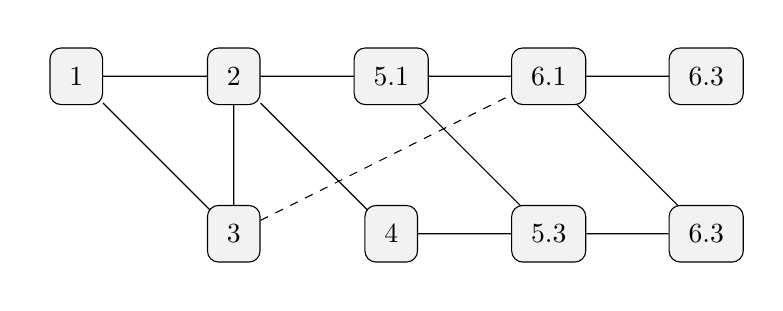
\begin{tikzpicture}[%
  chap/.style={fill=gray!10,draw,rounded corners,inner sep=7pt},
  w/.style={anchor=west},
  >=latex]
  \draw[] (0,0) node[chap] (c1) {1}
  --++(2,0) node[chap] (c2) {2} (c1) -- ++(2,-2) node[chap] (c3) {3}
  (c2) --++(2,-2) node[chap] (c4) {4}
  (c2) --++(2,0) node[chap] (c51) {5.1} --++(2,-2) node[chap] (c52) {5.3}
  (c51) --++(2,0) node[chap] (c61) {6.1} --++(2,-2) node[chap] (c62) {6.3}
  (c61) --++(2,0) node[chap] (c63) {6.3}
  (c4) -- (c52) -- (c62) (c3) -- (c2);
  \draw[dashed] (c3) -- (c61);
  \node at (-.5,.5) {}; \node at (8.5,-2.5) {};
\end{tikzpicture}
\end{document}


%%% Local Variables:
%%% mode: latex
%%% TeX-master: t
%%% End:
